\subsection{Optimierung unter Nebenbedingungen (KKT)}

Erweiterung des Lagrange-Verfahrens um Nebenbedingungen.
Es gelten folgende KKT-Bedingungen:

\begin{enumerate}[label=(\Roman*)]
    \item \(g_i(x^*)\leq 0 \rightarrow \) \emph{Ungleichungs-NB nach \(0\) umformen}
    \item \(h_j(x^*)=0 \rightarrow\) \emph{Gleichungs-NB nach \(0\) umformen}
    \item \(\lambda_i^*\geq 0\)
    \item \(\lambda_i^*g_i(x^*)=0\)
    \item $\mathcal{L}'(x,\lambda, v) = \nabla f(x^*) + \sum_{i=1}^m \lambda_i^* \nabla g_i(x^*) + \sum_{j=1}^p v_j^* \nabla h_j(x^*) = 0$
\end{enumerate}

mit den Lagrangemultiplikatoren ($\lambda, v$) als \emph{duale Variablen} und $x$ als \emph{primale Variable}.\\

\underline{Vorgehensweise}:
\begin{itemize}
    \item Gleichungs-NB vorhanden \(\rightarrow\) (II) nach einer Variablen auflösen und in (I) und (V) einsetzen
    \item 1. Ableitungen (Gradient \(\nabla\)) von (I), (II) und Zielfunktion \(f(x^*)\) bilden und (V) aufstellen
    \item (IV) aufstellen und Fallgruppen bilden: Was muss für \(\lambda_i\) und \(g_i(x^*)\) gelten, damit Produkt \(=0\) wird?
    \item Fallgruppen in (V) einsetzen und prüfen: Ist Lösung möglich? Sind alle Bedingungen erfüllt? Wenn ja: KKT-Punkt = Lösung gefunden; wenn nein: Kombination nicht zulässig \(\rightarrow\) verwerfen!
    \item Lösung: KKT-Punkt (\(x, y\)), Zielfunktionswert (\(p^*\)), duale Variablen (Lagrange-Multiplikatoren \(\lambda_i, v_j\))
\end{itemize}

\underline{Beispiel}:
\begin{align*}
    p^* &= \min 3x^2 + y^2\\
    \text{unter } x - y &\leq -8\\
    -y &\leq 0\\
\end{align*}

\begin{enumerate}
    \item \(g_1(x^*)=x-y+8 \leq 0 \rightarrow \nabla g_1(x^*) = \begin{pmatrix}
        1\\-1
    \end{pmatrix}\)\\
    \(g_2(x^*)=-y \leq 0 \rightarrow \nabla g_2(x^*) = \begin{pmatrix}
        0\\-1
    \end{pmatrix}\)\\
    \(\nabla f(x^*) = \begin{pmatrix}
        6x\\2y
    \end{pmatrix}\)\\

    \item (V): \(\begin{pmatrix}
        6x\\2y
    \end{pmatrix} + \lambda_1^* \begin{pmatrix}
        1\\-1
    \end{pmatrix} + \lambda_2^* \begin{pmatrix}
        0\\-1
    \end{pmatrix} = \begin{pmatrix}
        0\\0
    \end{pmatrix}\)\\

    \item \(\lambda_1^* g_1(x^*) = \lambda_1^*(x-y+8)=0 \rightarrow\) \underline{\(\lambda_1^*=0\)} und \(x-y+8=0 \Leftrightarrow \)\underline{\(x = y-8\)}\\
          \(\lambda_2^* g_2(x^*) = -\lambda_2^* y = 0 \rightarrow\) \underline{\(\lambda_2^*=0\)} und \underline{\(y=0\)}\\
    
    \item Fallkombinationen prüfen:
        \begin{itemize}
            \item \underline{Fall 1}: \(\lambda_1^* = \lambda_2^* = 0 \rightarrow \begin{pmatrix}
                6x\\2y
                \end{pmatrix} = \begin{pmatrix}
                    0\\0
                \end{pmatrix}\Leftrightarrow x=y=0\) \Lightning \hspace{0.1em} wegen \(x-y\leq-8\)
            \item \underline{Fall 2}: \(\lambda_1^* = y = 0 \rightarrow \begin{pmatrix}
                6x\\0
                \end{pmatrix} + \lambda_2^* \begin{pmatrix}
                    0\\-1
                \end{pmatrix}
                 = \begin{pmatrix}
                    0\\0
                \end{pmatrix}\Leftrightarrow x=\lambda_2^*=0\) \Lightning \hspace{0.1em} wegen \(x-y\leq-8\)

            \item \underline{Fall 3}: \(x=y-8; \lambda_2^*=0 \rightarrow
                \begin{pmatrix}
                    6(y-8)\\2y
                \end{pmatrix} + \lambda_1^* \begin{pmatrix}
                    1\\-1
                \end{pmatrix} = \begin{pmatrix}
                    0\\0
                \end{pmatrix}\)\\
                \begin{align*}
                    6y-48+\lambda_1^* &= 0\\
                    2y-\lambda_1^* &= 0\\
                    \cline{1-2}
                    8y = 48 \Leftrightarrow y &= 6 \checkmark\\
                    x = y-8 \Leftrightarrow x &= -2 \checkmark\\
                    \lambda_1^* = 2y &= 12 \checkmark
                \end{align*} Es handelt sich um einen KKT-Punkt

                \item \underline{Fall 4}: \(x=y-8; y=0 \rightarrow \begin{pmatrix}
                    6(-8)\\0
                    \end{pmatrix} + \lambda_1^* \begin{pmatrix}
                        1\\-1
                    \end{pmatrix} + \lambda_2^* \begin{pmatrix}
                        0\\-1
                    \end{pmatrix}
                     = \begin{pmatrix}
                        0\\0
                    \end{pmatrix}\Leftrightarrow \lambda_1^*=48\) und \(-\lambda_1^* - \lambda_2^* = 0 \Leftrightarrow \lambda_2^*=-48\) \Lightning \hspace{0.1em} wegen (III)
    

        \end{itemize} 
    \item \underline{Lösung}: Der Punkt \((x^*, y^*, \lambda_1^*, \lambda_2^2) = (-2, 6, 12, 0)\) erfüllt die KKT-Bedingungen (KKT-Punkt). \((x, y)=(-2,6)\) löst das \emph{primale Problem} und \((\lambda_1, \lambda_2)=(12,0)\) löst das \emph{duale Problem}. Damit ist \(p^*=3\cdot (-2)^2+6^2=48\)\\
\end{enumerate}


\subsection{Support Vector Machines (SVM)}

\begin{minipage}{0.4\textwidth}
    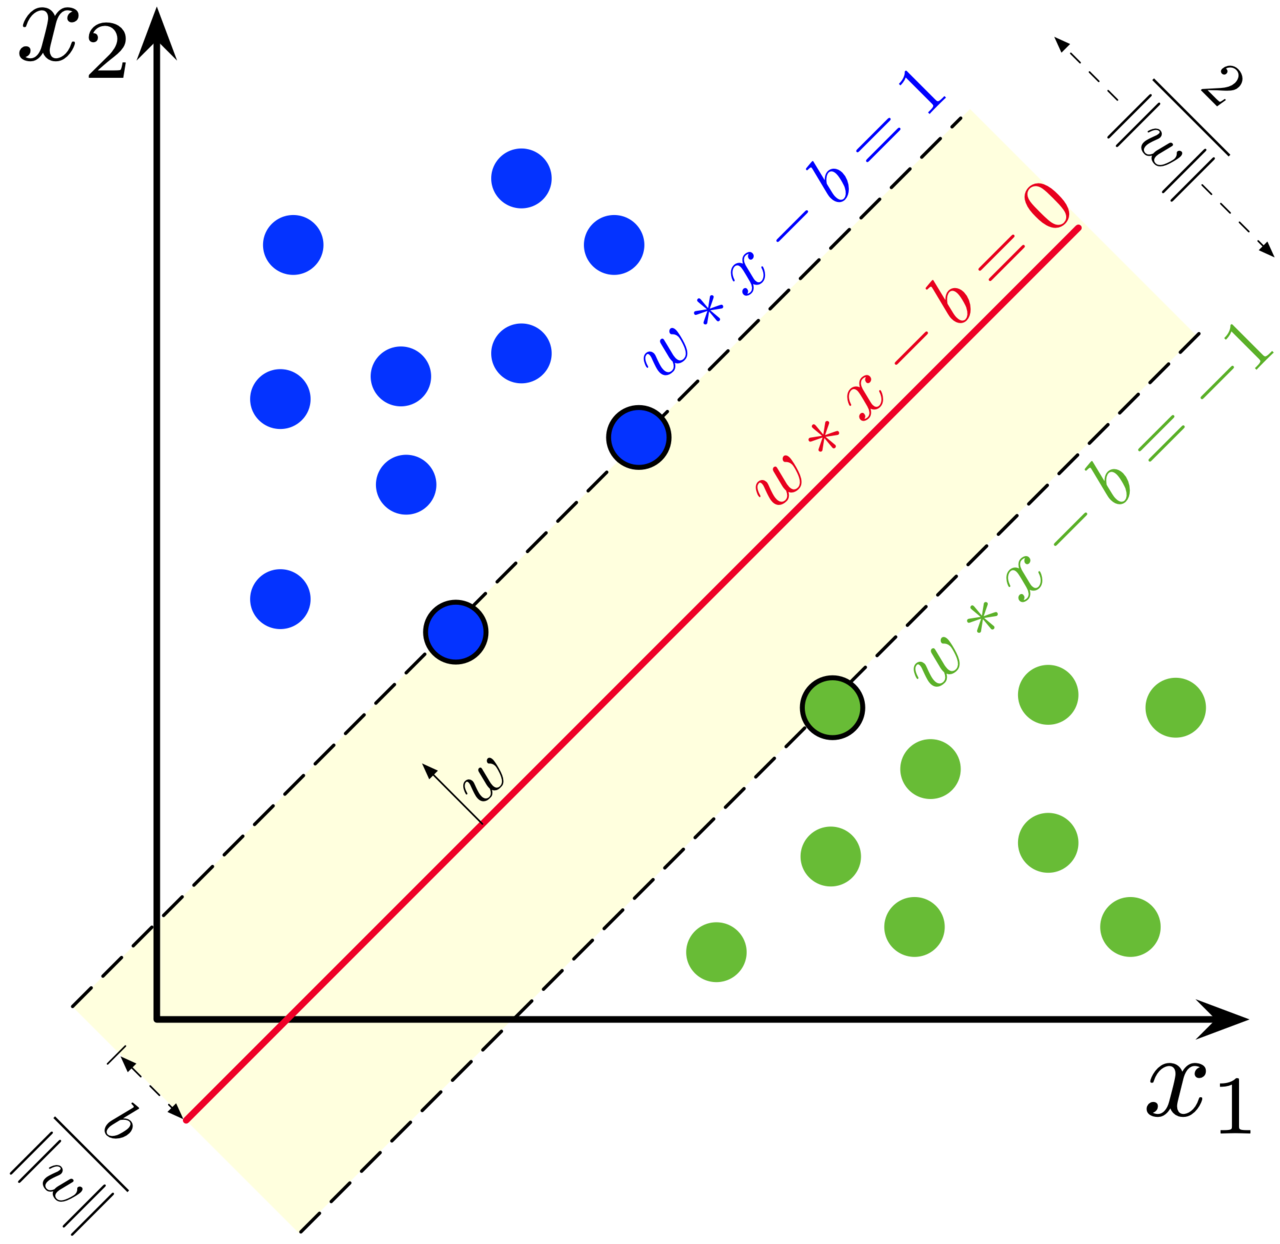
\includegraphics[width=\linewidth]{optimierung/SVM_margin.png}
\end{minipage}
\hfill
\begin{minipage}{0.5\textwidth}
    \begin{itemize}
        \item \underline{Ziel}: Finde die \emph{Hyperebene (Hyperplane)} mit der größten \emph{Geometric Margin} (Abstand zu den \emph{Support Vectors}). Da die \emph{margin-Breite} \(=\frac{2}{||w||}\) maximiert werden soll, wird \(||w||\) minimiert
        \item \emph{Support Vectors} sind die Punkte, die den \emph{Geometric Margin} bestimmen und selbst darauf liegen; alle anderen Punkte sind irrelevant
        \item \emph{Geometric Margin} ist der Abstand von der \emph{Hyperplane} zu den \emph{Support Vectors}
        \item \emph{Hyperplane} ist die Trennebene, die die Klassen voneinander trennt
    \end{itemize}
\end{minipage}
